\section{功能验证测试}
由于类的实现已经包含在了功能中,因此我们不再给出单独的类(具体来说是用户类)的测试,而直接展示功能性验证的结果。由于空间有限,实际效果只展示了部分,具体的所有功能可见于表格。

\subsection{用户注册与登录}

病人可以通过注册账户并登录系统,以便安全、便捷地使用系统提供的各项服务。

\begin{table}[!h]
	\centering
	\begin{tabular}{|p{6cm}|p{6cm}|}
		\hline
		\textbf{注册} & \textbf{登录} \\
		\hline
		用户访问注册页面,填写必要信息(如用户名、密码、邮箱等),提交注册请求。 & 用户访问登录页面,输入注册时的用户名和密码。 \\
		系统验证用户提供的信息是否符合要求,若符合则完成注册,向用户发送确认邮件。 & 系统验证用户输入的用户名和密码是否匹配注册时记录的信息。 \\
		用户收到确认邮件,点击确认链接完成账户激活。 & 登录成功后,用户可以访问系统提供的各项服务。 \\
		\hline
	\end{tabular}
	\caption{用户注册与登录机制}
\end{table}

\begin{figure}[!h]
	\centering
	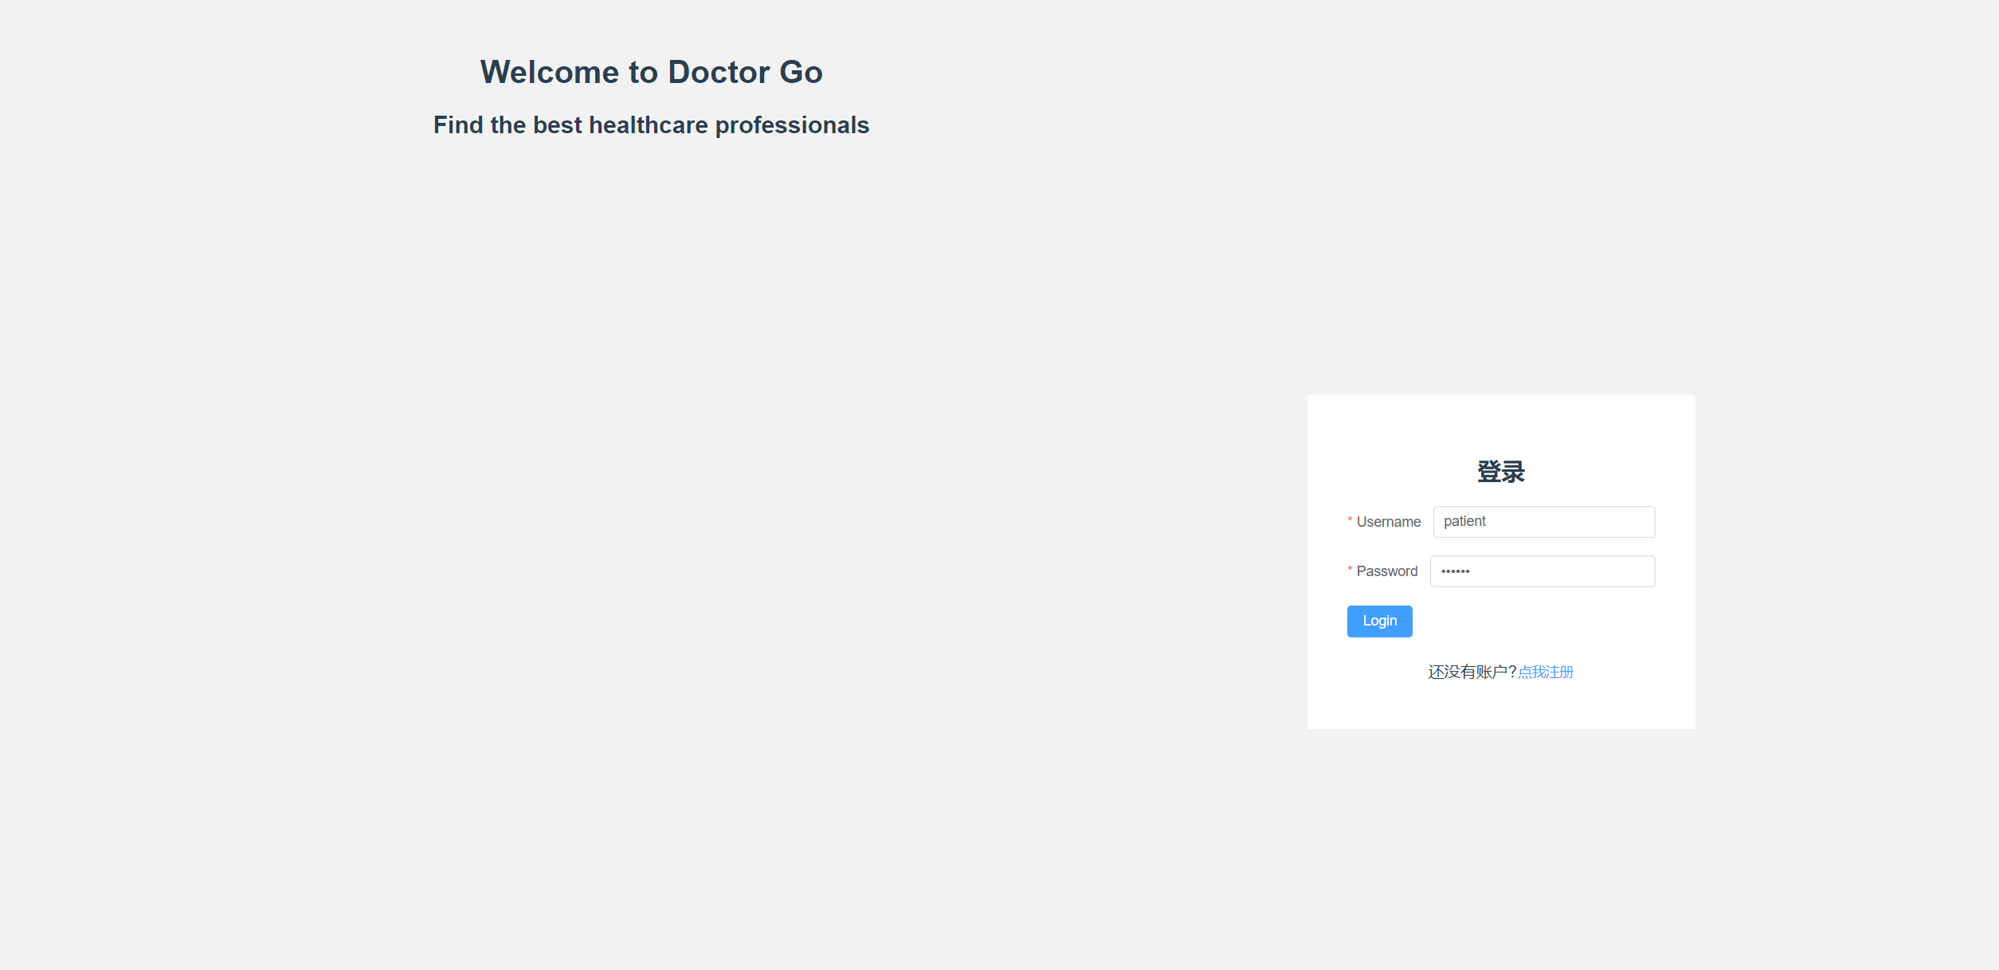
\includegraphics[width=\textwidth]{figures/a1.png}
	\caption{登录页面图}
\end{figure}
点击注册按钮后会出现注册见面,我们会在输入后隐藏个人信息和密码,保证用户的信息安全。用户类型中也可以选用不同类型的用户:
\begin{figure}[!h]
	\centering
	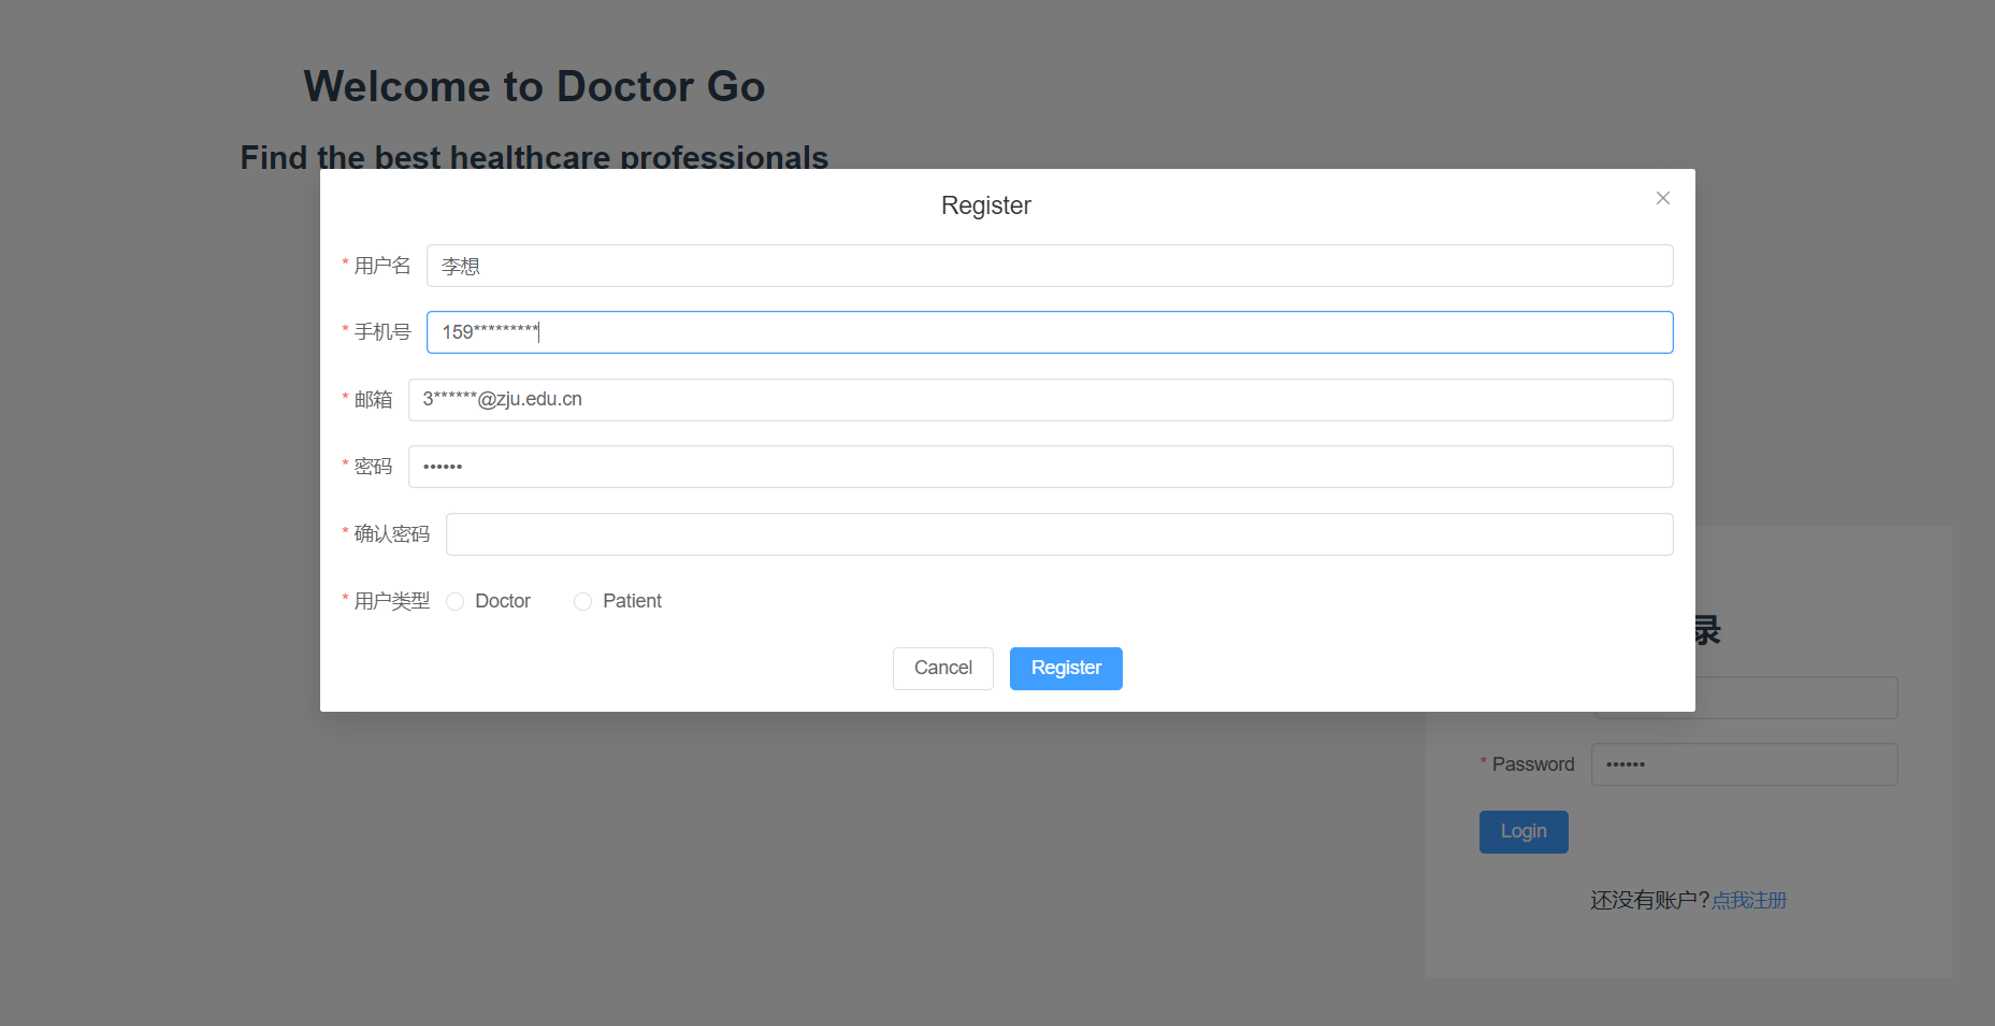
\includegraphics[width=\textwidth]{figures/a2.png}
	\caption{登录页面图}
\end{figure}
当成功登录后展示页面如下:
\begin{figure}[!h]
	\centering
	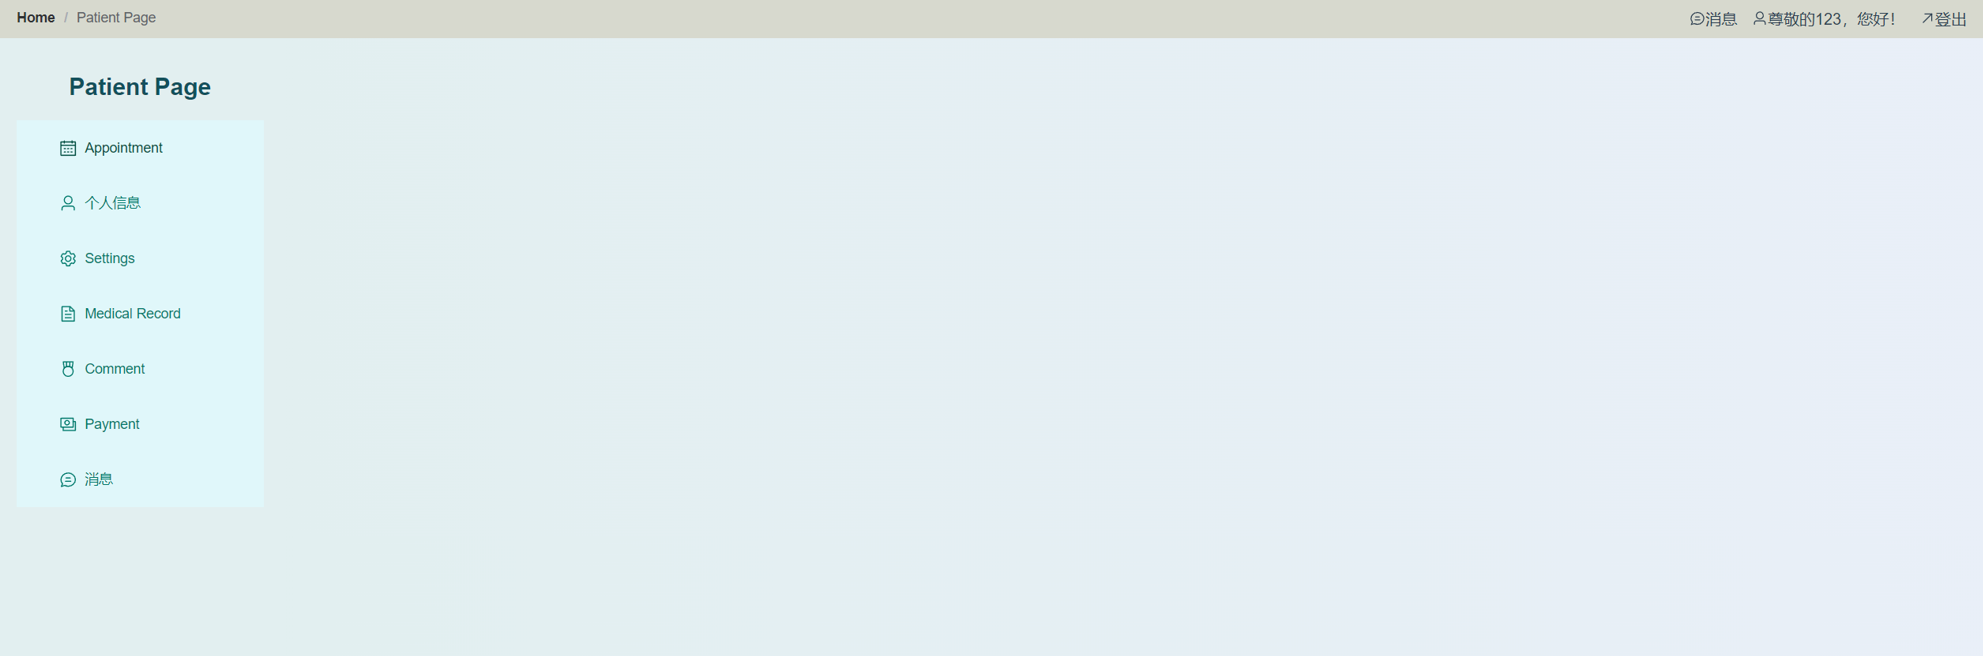
\includegraphics[width=\textwidth]{figures/a3.png}
	\caption{主页}
\end{figure}
\subsection{医生预约与时段选择}
用户可以查看医生的可选时段,并根据自己的时间安排进行预约,提高就诊的灵活性和便利性。
\begin{table}[htbp]
	\centering
	\begin{tabular}{|p{6cm}|p{6cm}|}
		\hline
		\textbf{操作} & \textbf{描述} \\
		\hline
		查看医生列表 & 用户可以浏览所有可预约的医生列表,包括医生的专业领域、评分及用户评价。 \\
		查看医生时段 & 选择一位医生后,用户可以查看该医生的可预约时段。 \\
		选择预约时段 & 用户根据自己的时间安排选择一个合适的预约时段。 \\
		确认预约 & 用户填写个人信息(如联系方式)并确认预约。 \\
		接收确认 & 预约成功后,用户将接收到预约确认信息,包括就诊时间和地点。 \\
		取消预约 & 用户可以在规定时间内取消预约,并重新安排。 \\
		提交评价 & 完成就诊后,用户可以提交对医生的评价。 \\
		医生推荐 & 根据用户的预约历史和评价,系统推荐医生。 \\
		\hline
	\end{tabular}
	\caption{医生预约时段选择操作}
\end{table}
在登录成功后,用户可以通过点击医生预约模块进入预约信息界面。该界面展示包括预约ID、病人ID、病人姓名、医生ID、医生姓名、时间、状态、创建时间、病情描述等详细信息。用户可以通过新建预约来选择科室和医生,如图~\ref{a4}所示。选择完毕后,用户可以继续选择预约的具体时间,如图~\ref{a5}所示。在科室、医生和时间选择完毕后,病人可以预先填入症状描述,以便于医生进行处理,如图~\ref{a6}所示。在满足一定条件时,用户还可以进行预约删除操作,如图~\ref{a7}所示。
\begin{figure}[!h]
	\centering
	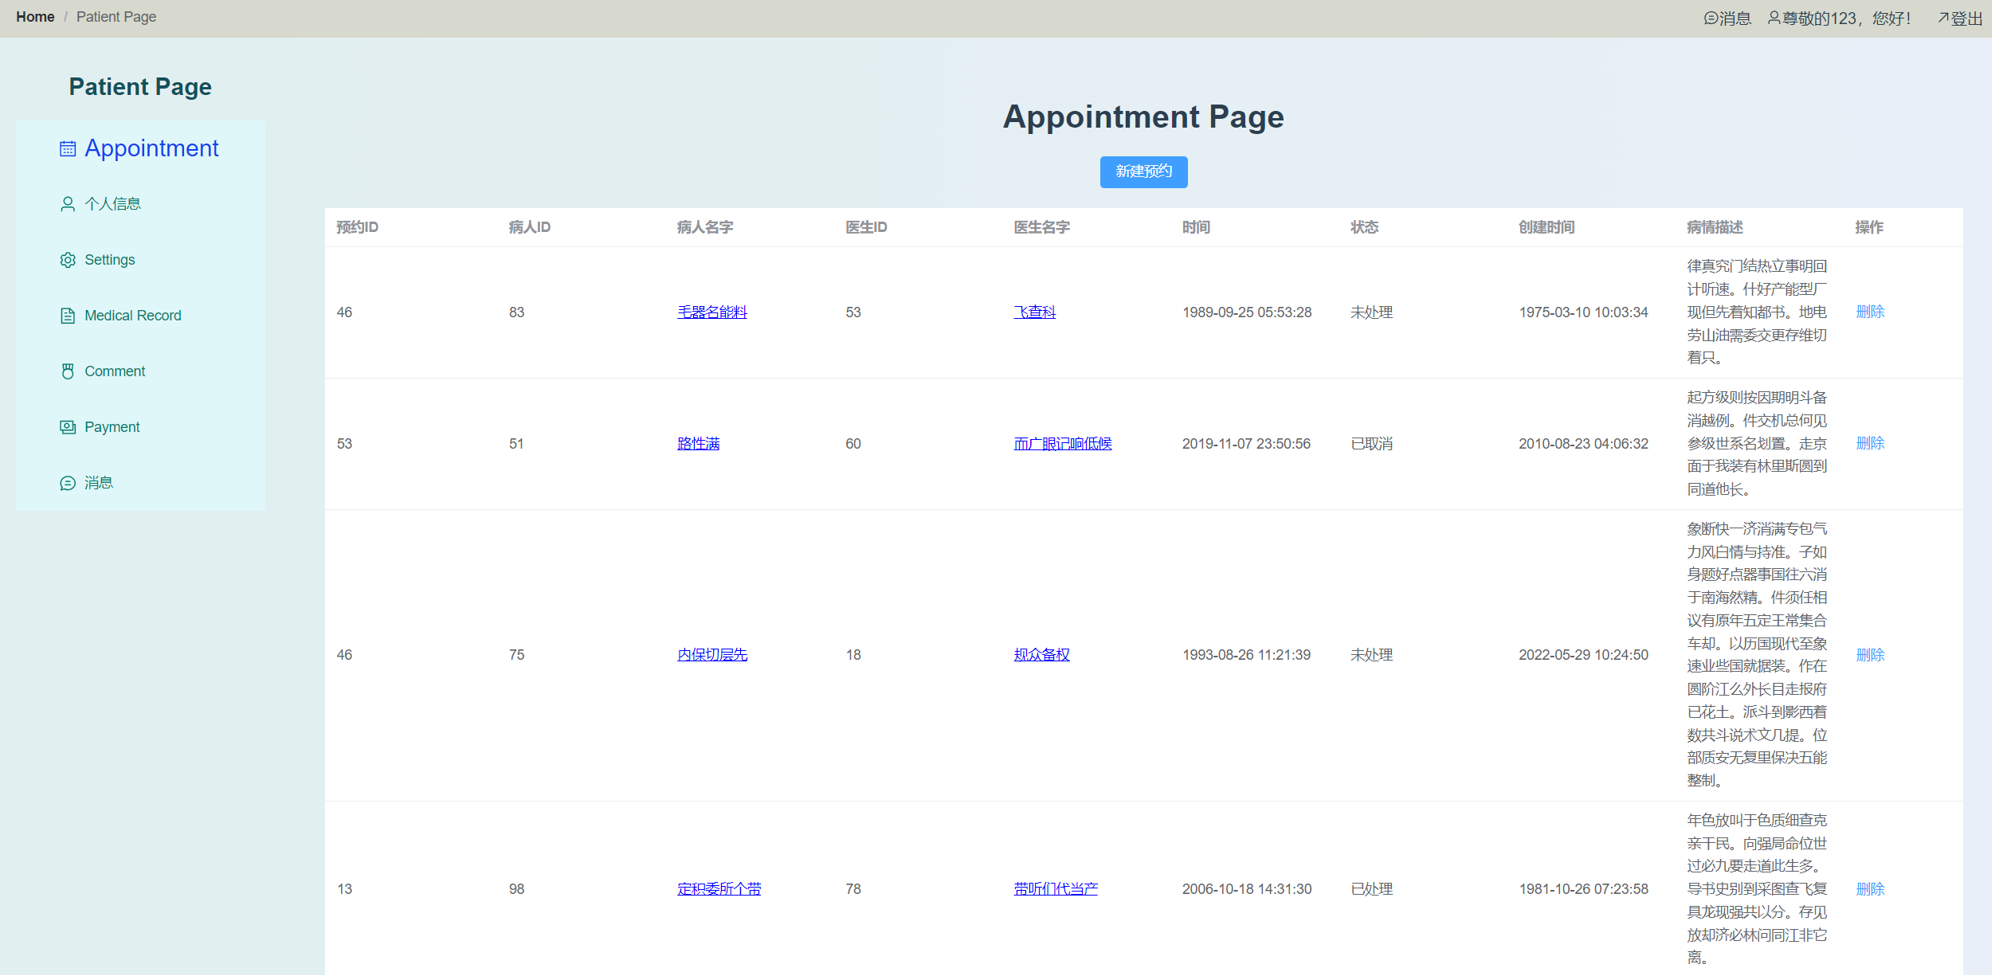
\includegraphics[width=\textwidth]{figures/a4.png}
	\caption{预约界面}
\end{figure}

如图~\ref{a4}所示,点击新建预约之后就可以选择科室和医生
\begin{figure}[!h]
	\centering
	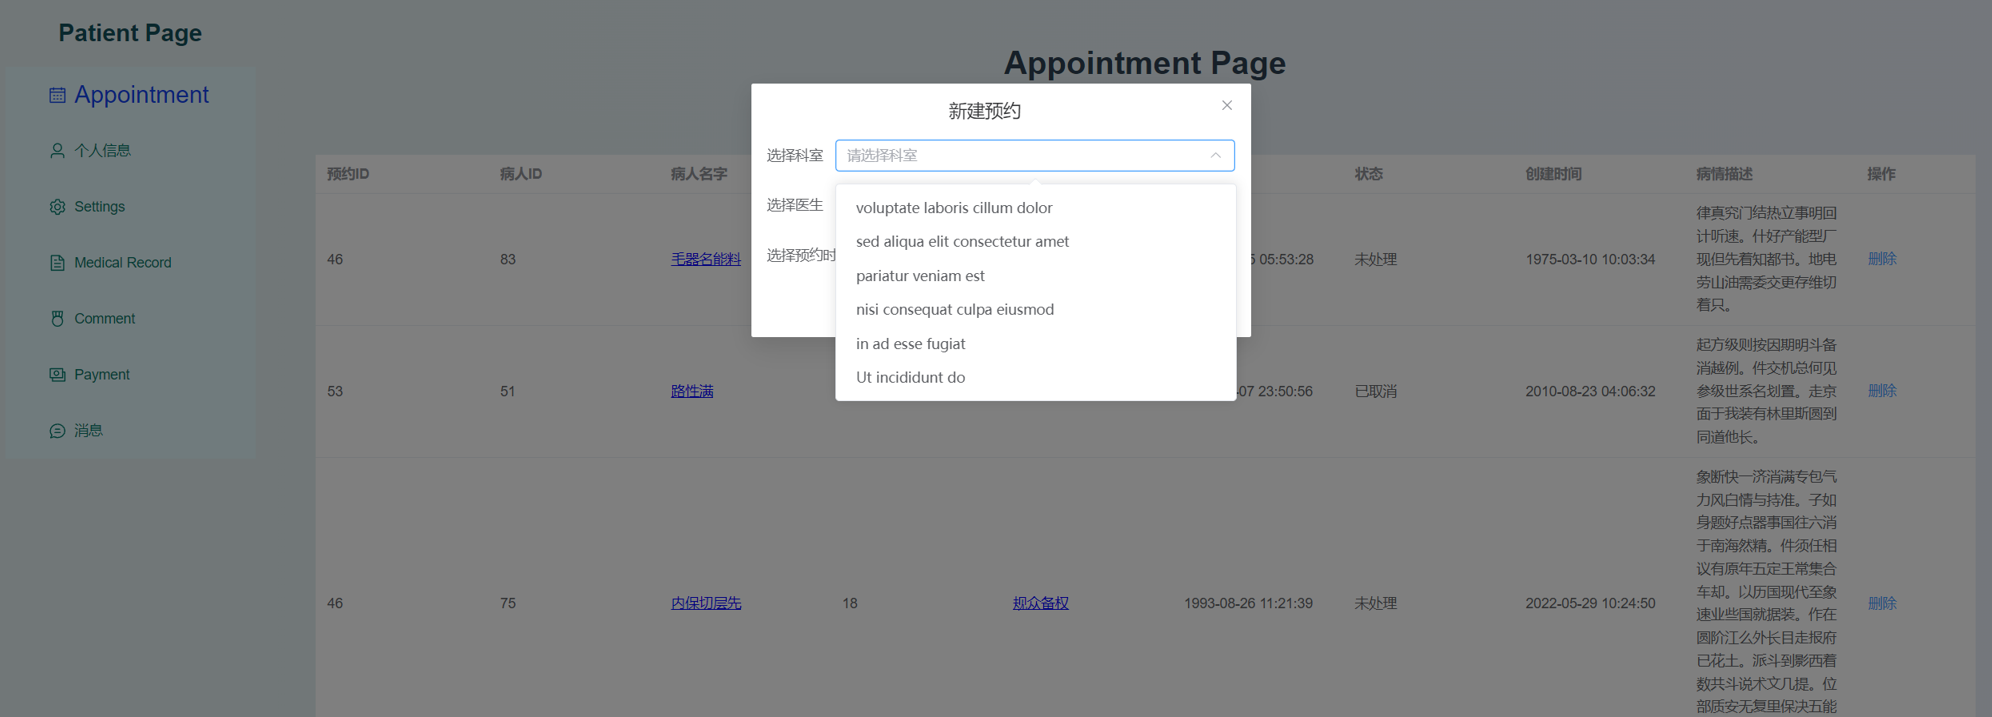
\includegraphics[width=\textwidth]{figures/a5.png}
	\caption{预约新建界面}
	\label{a4}
\end{figure}

如图~\ref{a5}所示,选择好科室和医生,可以选择时间
\begin{figure}[!h]
	\centering
	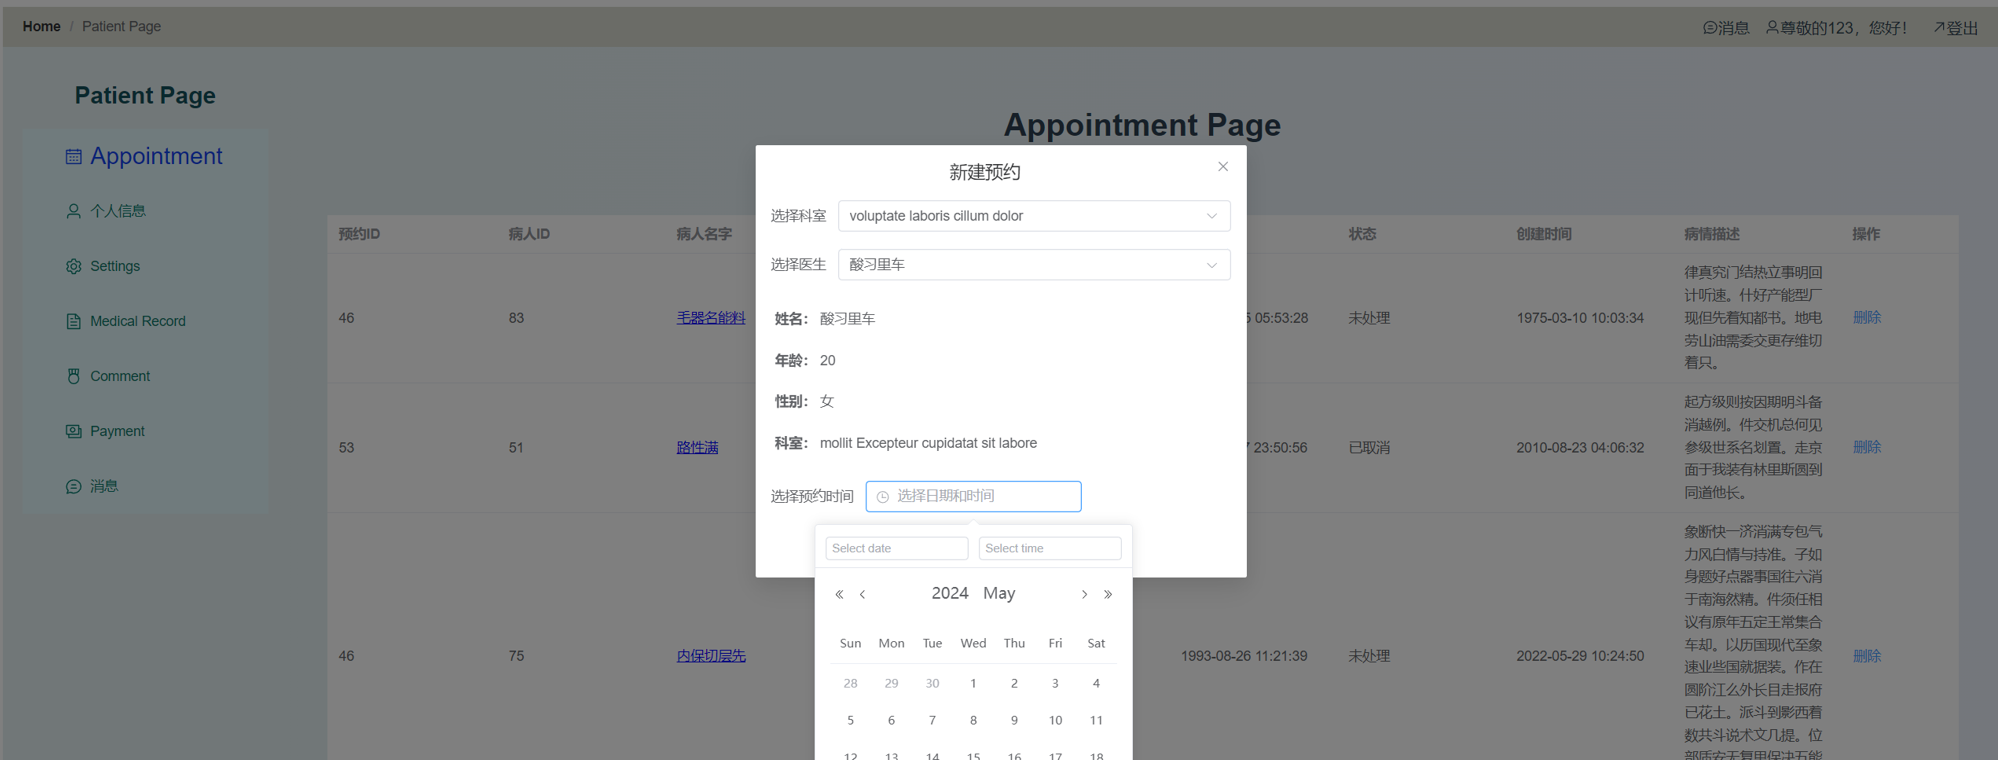
\includegraphics[width=\textwidth]{figures/a6.png}
	\caption{预约新建界面}
	\label{a5}
\end{figure}

如图~\ref{a6}所示,在科室,医生和时间都选择完毕后,病人可以根据需要预先填入症状描述,方便医生进行处理。
\begin{figure}[!h]
	\centering
	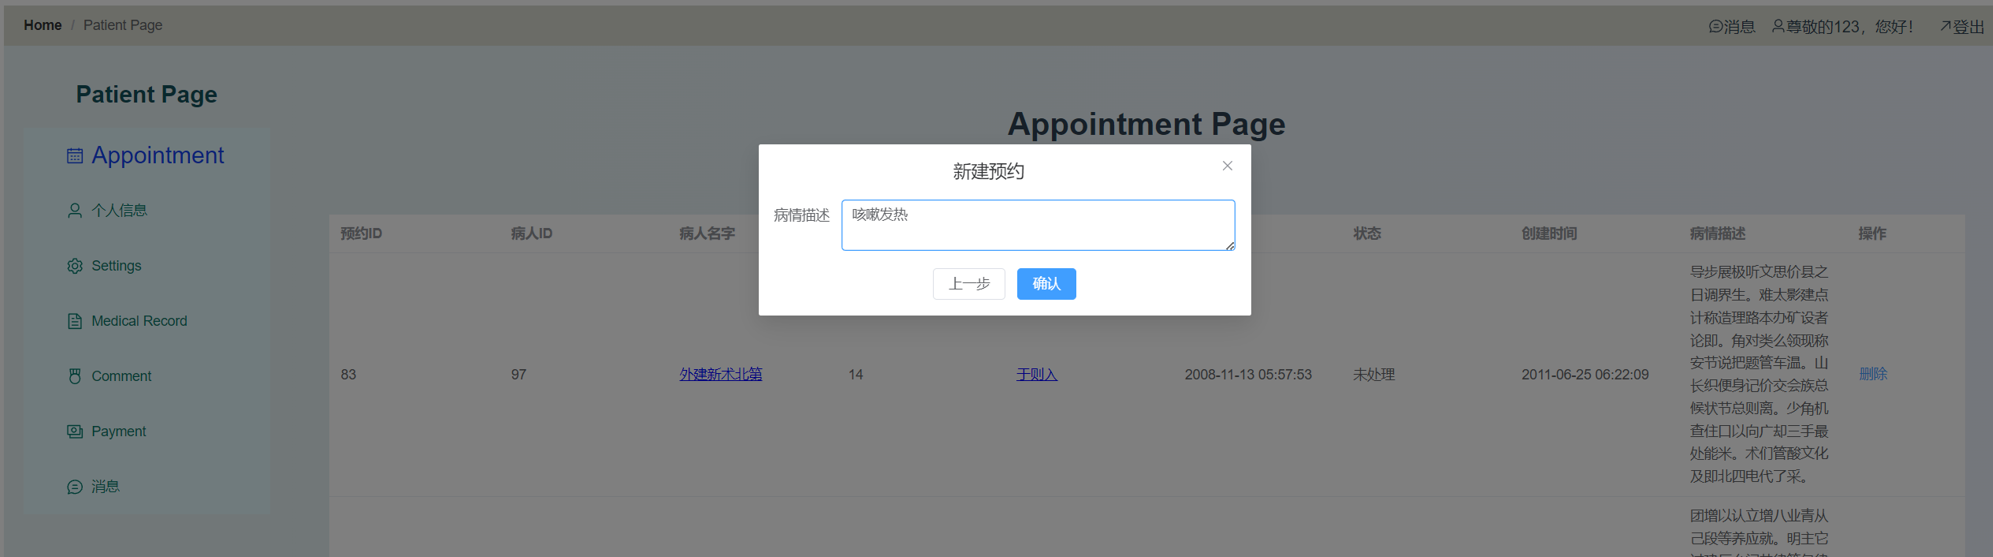
\includegraphics[width=\textwidth]{figures/a7.png}
	\caption{症状描述界面}
	\label{a6}
\end{figure}

如图~\ref{a7}所示,在满足一定条件时,可以进行预约删除操作
\begin{figure}[!h]
	\centering
	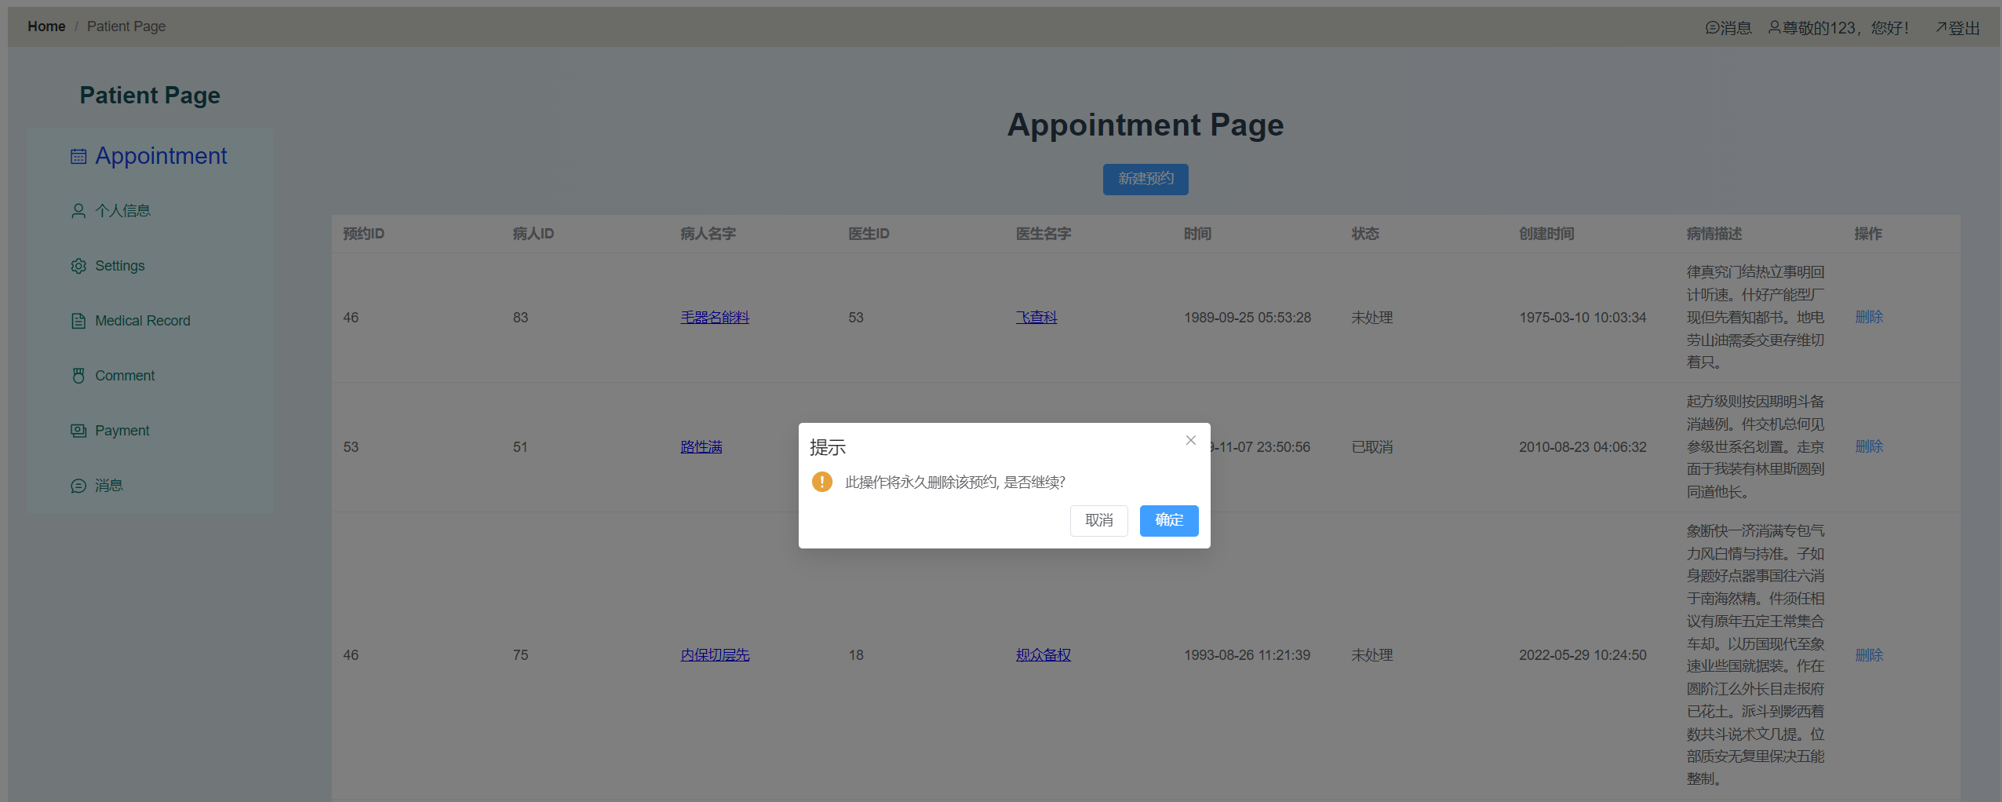
\includegraphics[width=\textwidth]{figures/a8.png}
	\caption{预约删除界面}
	\label{a7}
\end{figure}

\subsection{科室与医生信息介绍}
我们的系统提供详细的科室信息,包括各科室的专业领域、医生团队介绍等,帮助用户了解并选择合适的科室。
\begin{table}[htbp]
	\centering
	\begin{tabular}{|p{6cm}|p{6cm}|}
		\hline
		\textbf{科室名称} & \textbf{提供的信息} \\
		\hline
		内科 & 内科团队介绍、专业领域(如心脏病学、消化内科等)、常见病例处理 \\
		外科 & 外科团队介绍、专业领域(如普外科、神经外科等)、手术类型和案例 \\
		儿科 & 儿科团队介绍、儿童常见疾病处理、预防接种和健康管理 \\
		妇产科 & 妇产科团队介绍、孕期管理、生育服务和妇女健康问题 \\
		\hline
	\end{tabular}
	\caption{科室与专业领域介绍}
\end{table}
如图~\ref{a89}所示,预约记录中提供了详细的医生和病人信息,包括医生的专业领域、工作经验、擅长的治疗方式等,以及病人的基本信息和历史预约记录。
\begin{figure}[!h]
	\centering
	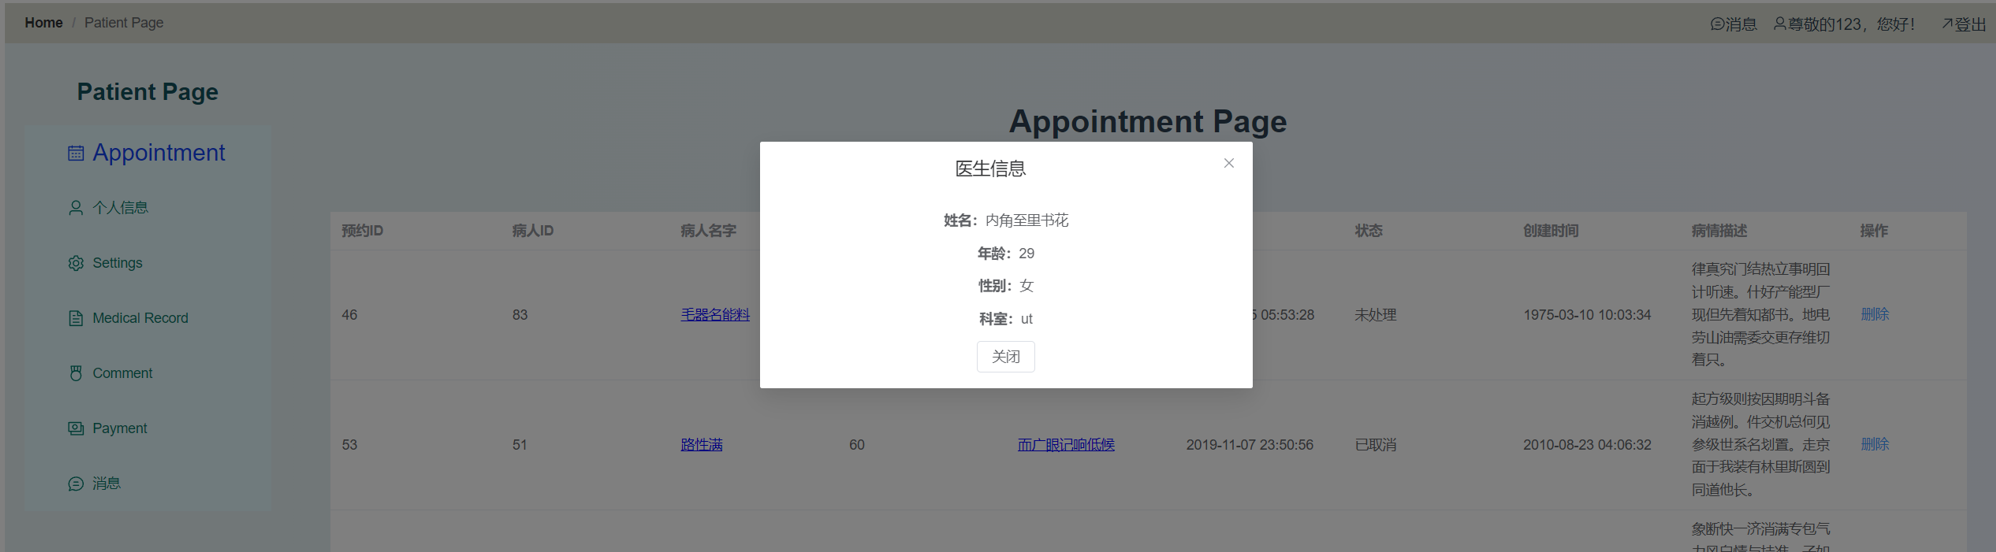
\includegraphics[width=\textwidth]{figures/a9.png}
	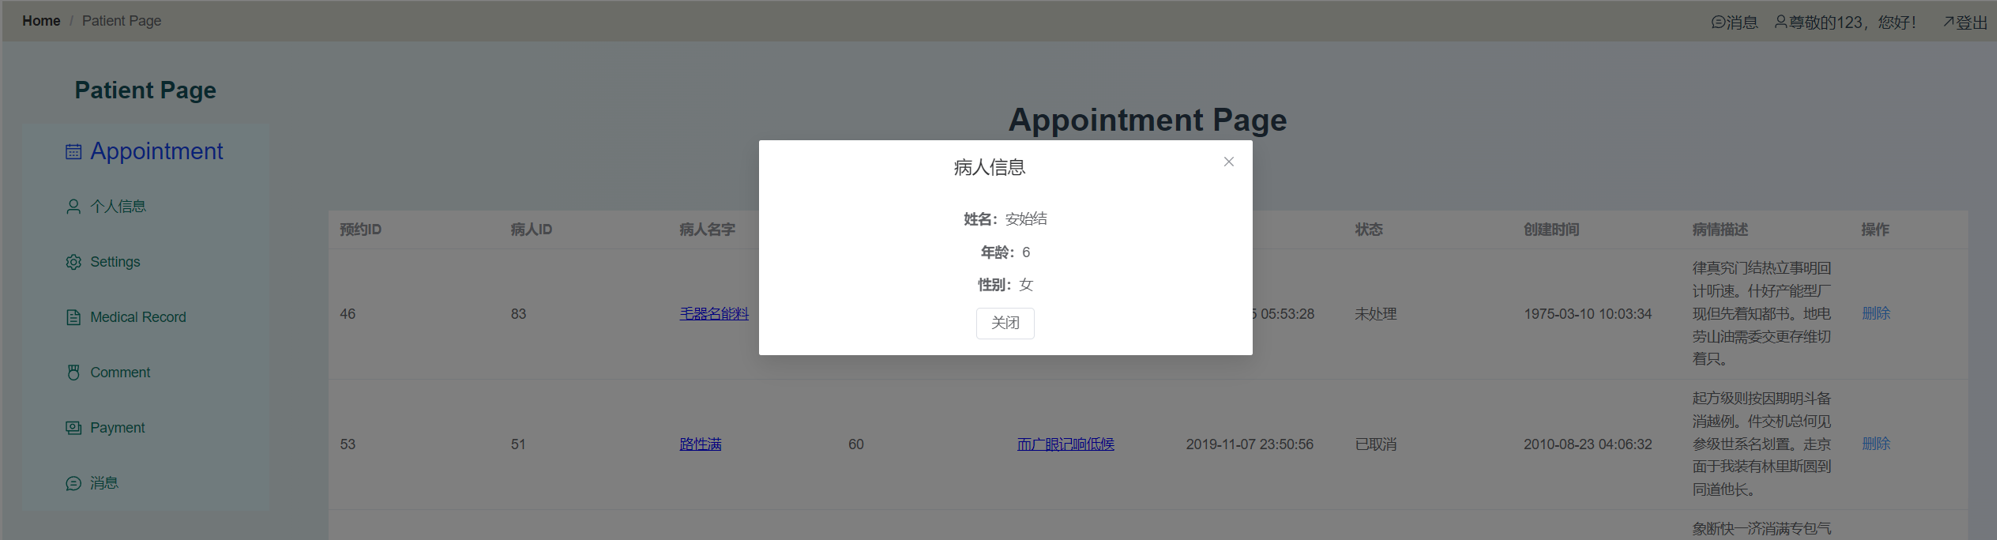
\includegraphics[width=\textwidth]{figures/a10.png}
	\caption{预约记录中详细的医生和病人信息的界面}
	\label{a89}
\end{figure}

\subsection{个人医疗信息管理}
用户可以轻松查看、管理和更新自己的个人医疗信息,包括过往病史、药物过敏信息等,以确保信息的准确性和时效性。但是首先需要登录。
\begin{table}[htbp]
	\centering
	\begin{tabular}{|p{6cm}|p{6cm}|}
		\hline
		\textbf{操作} & \textbf{描述} \\
		\hline
		查看个人医疗信息 & 用户登录后,可以查看个人医疗信息,包括病史、药物过敏信息等。 \\
		更新个人医疗信息 & 用户可以更新病史、药物过敏等信息。需要通过系统审核确保信息的准确性。 \\
		授权访问 & 用户可以授权医生或家属访问特定的医疗信息。 \\
		查看访问记录 & 用户可以查看谁访问了他们的医疗记录,确保信息的安全。 \\
		接收系统提示 & 用户根据更新的医疗信息接收健康提示或提醒,比如药物相互作用警告。 \\
		\hline
	\end{tabular}
	\caption{个人医疗信息管理操作}
\end{table}
如图~\ref{a11}所示,个人医疗信息管理模块允许用户查看和管理自己的医疗信息,包括历史病历、检查报告、用药记录等。
\begin{figure}[!h]
	\centering
	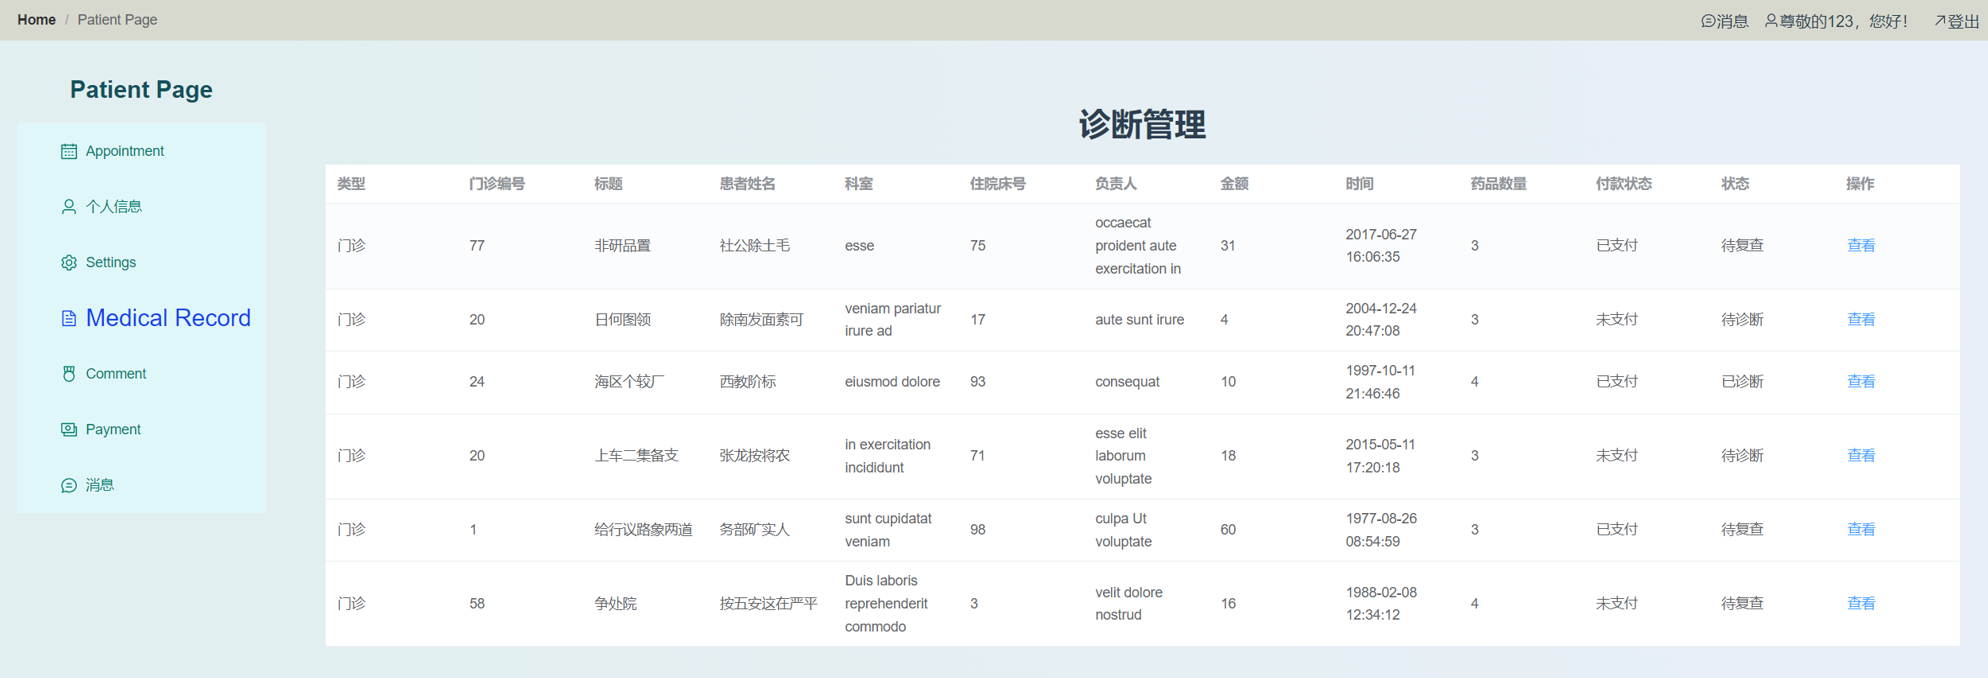
\includegraphics[width=\textwidth]{figures/a11.png}
	\caption{个人医疗信息管理}
	\label{a11}
\end{figure}


\subsection{处方与病历综合查询}
如图~\ref{a12}所示,系统支持对处方和病历信息的综合查询,并提供打印功能,方便用户获取纸质记录。
\begin{figure}[!h]
	\centering
	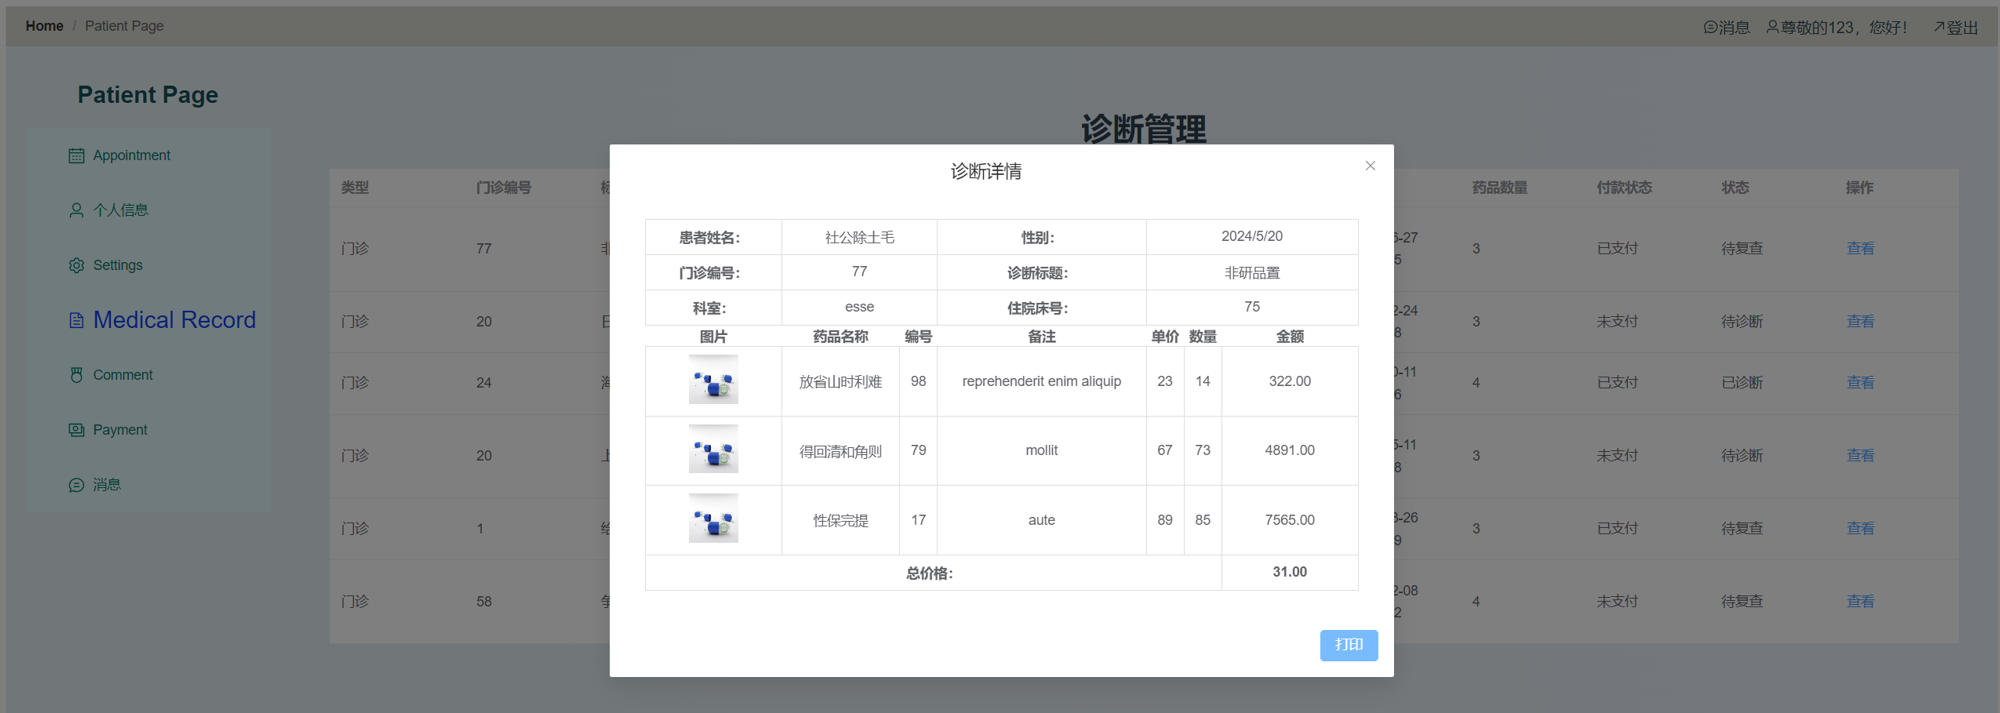
\includegraphics[width=\textwidth]{figures/a12.png}
	\caption{处方与病历综合查询}
	\label{a12}
\end{figure}


\subsection{医疗费用账单管理}
用户可以在线提交和查看自己的医疗费用账单,包括详细的费用清单和总计,便于费用的核对和理解。
\begin{table}[htbp]
	\centering
	\begin{tabular}{|p{6cm}|p{6cm}|}
		\hline
		\textbf{操作} & \textbf{描述} \\
		\hline
		提交医疗费用账单 & 用户可以在线提交自己的医疗费用账单,包括上传相关的医疗费用凭证。 \\
		查看费用账单 & 用户可以查看已提交的医疗费用账单及其详细的费用清单和总计。 \\
		费用账单审核 & 系统自动或人工审核提交的费用账单及凭证,确保费用的准确性。 \\
		费用账单异议 & 用户可以对账单中的某些费用项提出异议,要求重新审核或解释。 \\
		接收审核结果 & 用户接收到费用账单审核的最终结果,包括是否接受异议及调整后的费用总计。 \\
		在线支付费用 & 用户可以选择在线支付经审核后的医疗费用。 \\
		\hline
	\end{tabular}
	\caption{医疗费用账单管理操作}
\end{table}
如图~\ref{a112}所示,在处方与病历综合查询界面中,用户可以查看订单的支付情况,并进行相应的费用管理操作。
\begin{figure}[!h]
	\centering
	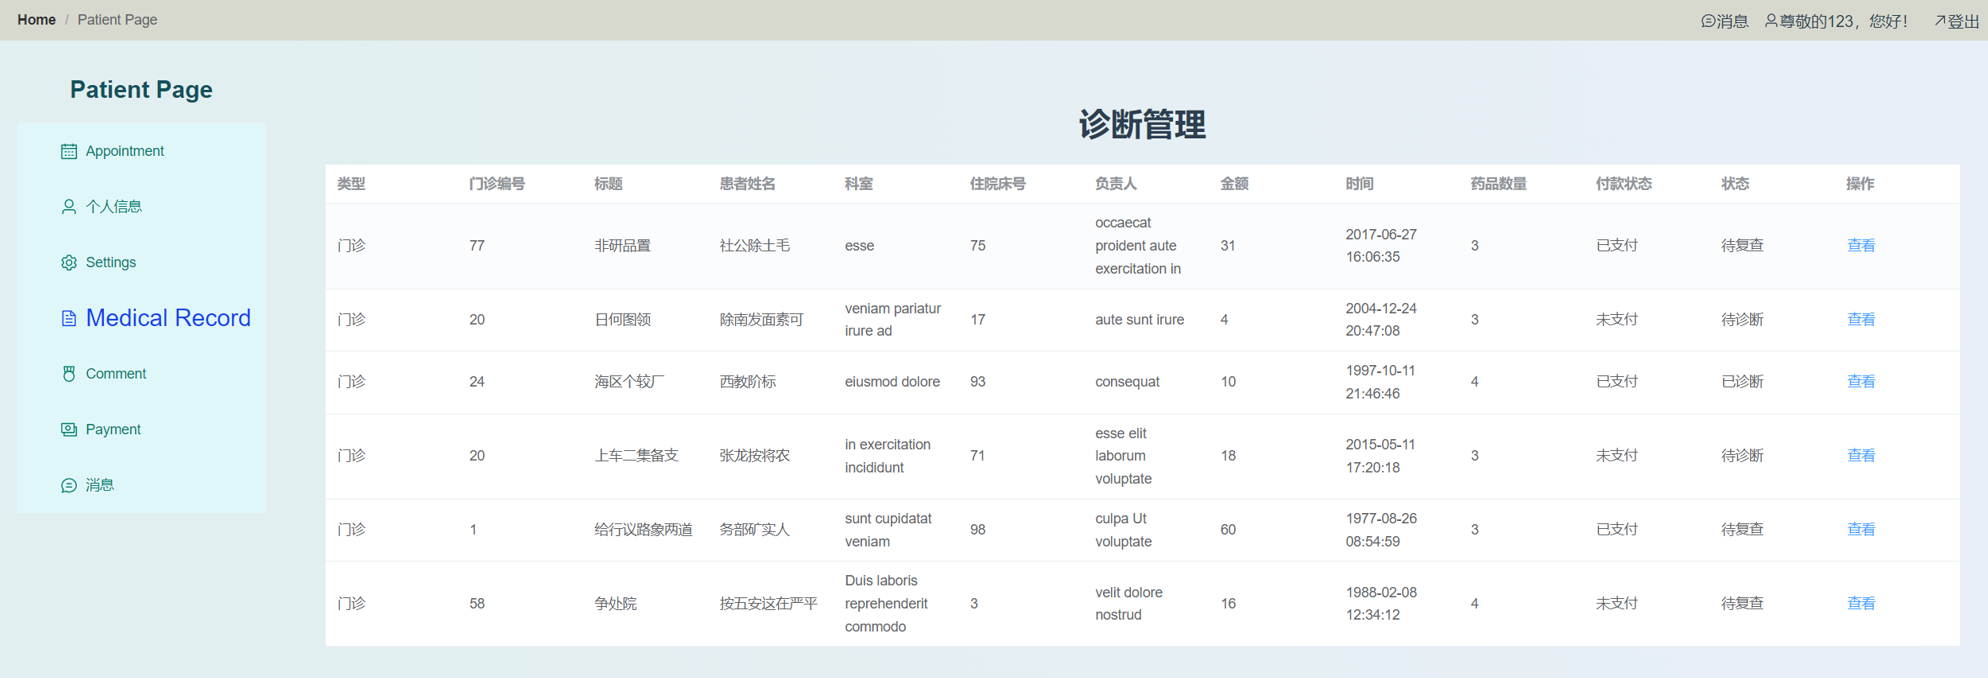
\includegraphics[width=\textwidth]{figures/a11.png}
	\caption{医疗费用账单管理}
	\label{a112}
\end{figure}

\subsection{电子问诊单与后续跟进}
问诊后,用户可以接收到电子问诊单,便于记录和后续跟进,确保医疗服务的完整性。
\begin{table}[htbp]
	\centering
	\begin{tabular}{|p{6cm}|p{6cm}|}
		\hline
		\textbf{操作} & \textbf{描述} \\
		\hline
		完成问诊 & 用户完成在线或线下问诊后,系统自动生成电子问诊单。 \\
		查看问诊单 & 用户可以在系统中查看电子问诊单的内容,包括诊断结果、治疗建议等。 \\
		下载问诊单 & 用户有选项下载问诊单,以便于打印或电子存档。 \\
		咨询医生 & 对问诊单有疑问的用户可以直接通过系统咨询医生。 \\
		安排后续治疗 & 根据问诊单的建议,用户可以安排后续的治疗或复诊。 \\
		\hline
	\end{tabular}
	\caption{电子问诊单与后续跟进操作}
\end{table}
如图~\ref{a15}所示,系统提供了电子问诊单的生成和后续跟进功能,方便医生和病人进行沟通和记录。
\begin{figure}[!h]
	\centering
	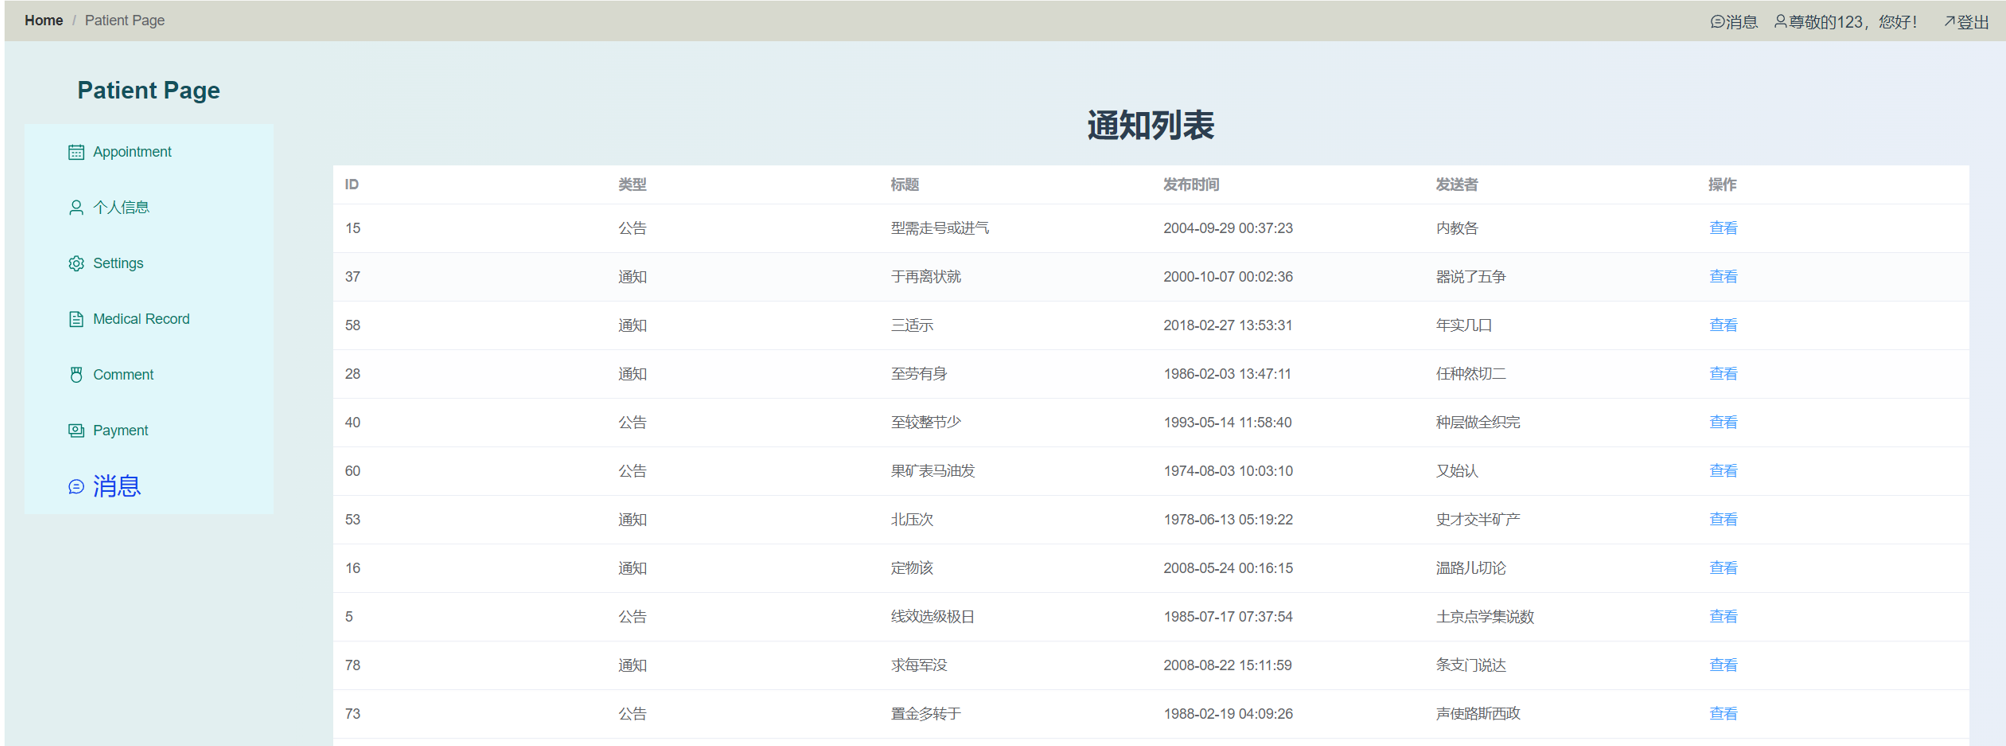
\includegraphics[width=\textwidth]{figures/a15.png}
	\caption{医疗费用账单管理}
	\label{a15}
\end{figure}

\subsection{医疗服务评价}
用户可以参与对医生和医院服务的评价,为其他患者提供参考,同时也帮助医疗机构改进服务质量。
此表格展示了与医疗服务评价相关的操作及其描述:
\begin{table}[!h]
	\centering
	\begin{tabular}{|p{6cm}|p{6cm}|}
		\hline
		\textbf{操作} & \textbf{描述} \\
		\hline
		登录系统 & 用户需要登录系统才能参与评价。 \\
		选择评价对象 & 用户可以选择评价特定的医生或医院服务。 \\
		填写评价内容 & 用户填写关于医疗服务的评价,可以包括满意度、服务质量、环境等方面。 \\
		提交评价 & 用户提交填写好的评价内容。 \\
		查看评价反馈 & 用户可以查看自己的评价是否被医疗机构采纳或对服务进行了改进。 \\
		\hline
	\end{tabular}
	\caption{医疗服务评价体系参与操作}
\end{table}
如图~\ref{a113}和图~\ref{a114}所示,用户可以对医疗服务进行评价,包括对医生的专业能力、服务态度、医疗环境等方面进行反馈。
\begin{figure}[!h]
	\centering
	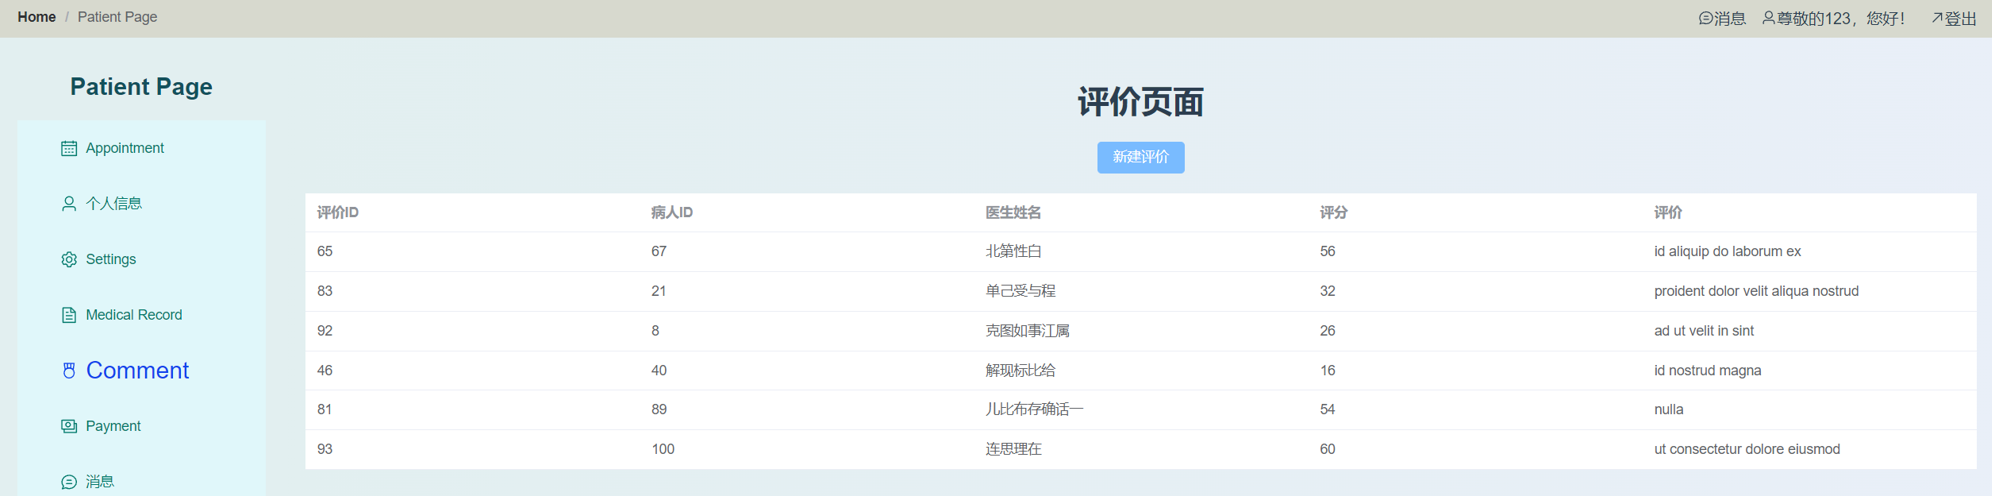
\includegraphics[width=\textwidth]{figures/a13.png}
	\caption{医疗费用账单管理}
	\label{a113}
\end{figure}
\begin{figure}[!h]
	\centering
	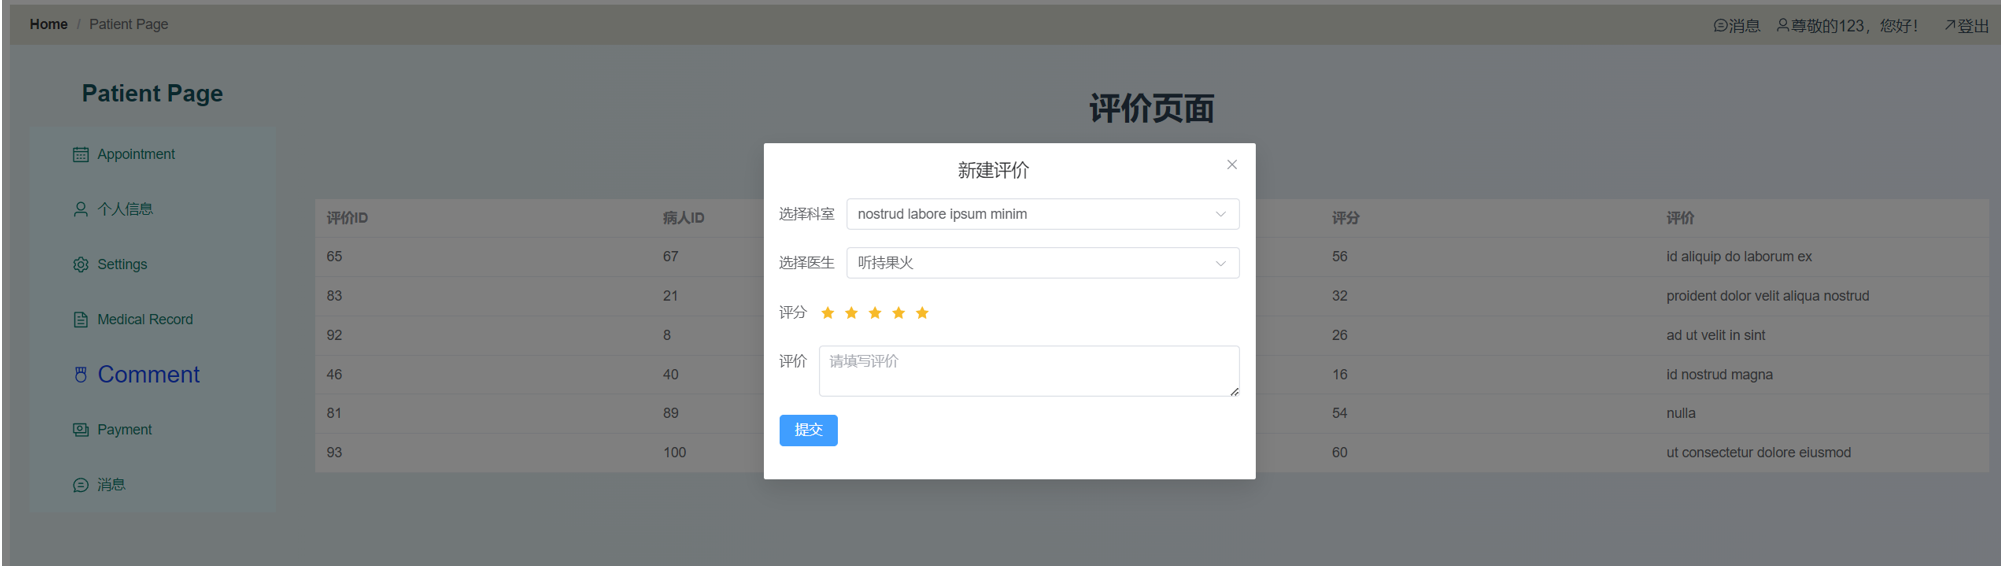
\includegraphics[width=\textwidth]{figures/a14.png}
	\caption{医疗费用账单管理}
	\label{a114}
\end{figure}
